% Chapter 1

\chapter{Introduction} % Write in your own chapter title
\label{Chapter1}
Image transfer over a low bandwidth channel has always been challenging
task. Specially, if image is taken from a live camera and it has to be
transmitted over a wireless delay tolerant network, then the task is further
twisted. Complexity increases further, if we need to build a viable low
cost system with a low power solution. In any such solution it would be
wise to transmit information only. Yes, information!!!  Information
about image!! We need to extract information out of image and then to
send it over the network.  Information can be of various type. So, we
need to deal that what minimum information about image allows us to
reconstruct the scenario or to detect an event. We also need to look
that how can these informations be represented so that it helps in
efficient system(SW/HW) development.Most appropriate application for
above technology can be smart video surveillance network.

\section{Motivation}

Most of the existing video surveillance system is still manual. Normally
all the surveillance camera video is sent to a monitoring base station,
where it is monitored by a person or a group of person. But such
arrangement can not be full proof. So, any attempt in the direction of
its automation can be of great use in following application areas:
\begin{enumerate}
 \item  Traffic Monitoring
  \item Elderly care
  \item Security
  \item Surveillance
  \item Assembly Line Inspection
\end{enumerate}

End goal of such an intelligent system would be to offer an
automatic analysis of scene and then to infer desired information out of
it.Such a system can be lot complex because of the complexity of the
scene, specially when application is targeted for outdoor monitoring.
Sometime background of the scene can be moving, while in some
other scene ambient light can be different. Similarly can be many other
hurdles in the process of automation. But if an efficient
background detection algorithm is chosen then, these issued can be
addressed up to a lot extent.



\section{Past Work and Literature Survey}

Overall this task can broadly be divided into two categories: Extraction
of information from images \& then representation of that information
through a semantic network.

\subsection{Extraction of Semantic information from Image}

Various research have been done to extract useful information from a
moving image. The toughest part of this implementation is to find an
efficient background estimation algorithm so that moving objects can be
identified. Features such as Gradient histogram, Gray Scale (Haar),
color, texture, self-similarity and motion have been used by different
researchers. \\ 
 ~\cite{1} and many other has used color information as the feature for
estimation. But only color as feature might not be sufficient ~\cite{2}
in surveillance applications where image resolution is very low.  Adding
motion along with image intensities gives better result in moving bodies
estimation. When background color is same as foreground color then
texture features represented by local binary pattern ~\cite{3} provides
interestingly nice result. Further, features computed at a single scale
can be used to approximate feature at nearby scale. Such implementations
~\cite{4} accelerates the execution for practical applications.
There is one implementation ~\cite{5} which decides about pixel that
whether it belongs to foreground or background dynamically.

Once all moving bodies have been separated out, then only points of
their contour or centroid can be sent over network.

\subsection{Representation of Semantic information}

\section{Issues and outstanding problems}

Methods of image transmission can broadly be divided into levels as shown
in \ref{fig1}. Most of these work have been done on lower three levels.
There are only few attempts on the upper layers ~\cite{6,7}.

\begin{figure}
\begin{center}
 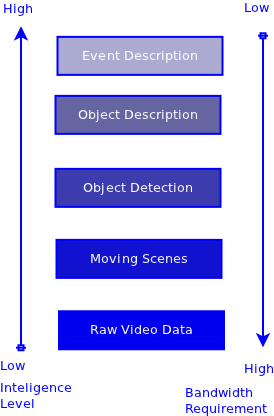
\includegraphics{../Figures/image_tr_level.png}
 % image_tr_level.png: 274x416 pixel, 72dpi, 9.67x14.68 cm, bb=0 0 274 416
 \caption{Lavel of Image Transfer}
 \label{fig1}
\end{center} 
\end{figure} 


\section{Approach}

A typical wireless sensor network can be as that of shown in figure
\ref{fig2}. Each node will have a camera, a processing engine and a
wireless transmission module. Transferring captured raw image will be
very expensive. Therefore they will be processed to
extract semantic information from it. Textual semantic information will
be transmitted over wireless media to the knowledge engine. Knowledge
engine will use ontology language such as OWL to represent these
information from different nodes. Such intelligent WSN can fit into many
important applications like security monitoring, elderly care etc.


\begin{figure}
\begin{center}
 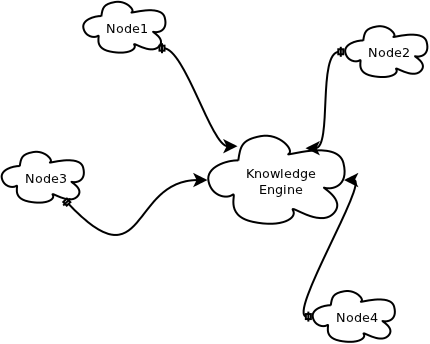
\includegraphics{../Figures/wsn.png}
 \caption{Wireless Sensor Network}
 \label{fig2}
\end{center} 
\end{figure} 


\section{Organisation of thesis}
